%\documentclass{minimal}
%
%\usepackage[pdftex,active,tightpage]{preview}
%\usepackage{tikz}
%\usepackage{pgfplots}
%\usetikzlibrary{plotmarks}
%
%\begin{document}
%\begin{preview}
\begin{figure}[tb]
	\centering
	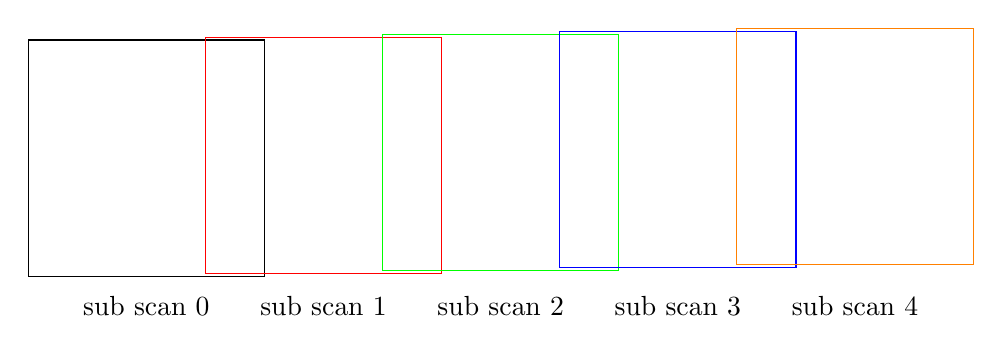
\begin{tikzpicture}[scale=.75]
		\foreach \x/\color in {0/black,
							1/red,
                         	2/green,
                         	3/blue,
                         	4/orange}
    	\draw[color=\color] (3*\x,.05*\x) rectangle (3*\x+4,.05*\x+4);
    	\foreach \x in {0,...,4}
   		\draw (3*\x+2,-.5) node [color=black] {sub scan \x};
	\end{tikzpicture}
	\caption{This should ultimatively explain the overlapping scans}
	\label{fig:overlapping scans}
\end{figure}

%\end{document}